\documentclass [12pt]{article}
\usepackage{amsmath}
\usepackage{color}
\usepackage{epstopdf}
\usepackage{graphicx}
\usepackage{pgfpages}
\usepackage{media9}
\setlength{\textwidth}{165mm} \setlength{\oddsidemargin}{0.0mm}
\setlength{\evensidemargin}{0.0mm}
\renewcommand \baselinestretch{1.2}




\begin{document}
\title{Block-Separable Copula Generated Random Graphs for Directed Networks\\}
\author{Jiguo Cao and Aaron J. Danielson\\}
\date{\today}
\maketitle


\begin{abstract}
\noindent 
Many methods exists to model networks.  In order to recreate complex patterns, methods like stochastic block models assign nodes to communities and estimate the probability of a tie within and between members of the groups.  Other methods, such as exponential random graph models (ERGMs), model the dependence explicitly via a vector of sufficient statistics.  This paper introduces a new class of network models we call copula generated random graphs (CGRGs) that borrows from both traditions.  After specifying the general model, we apply the model to two networks from different domains.  A real-valued network representing regulation in the brain's default mode network is modeled as a copula generated random graph.  The flexible structure allows for the model to account for differences between units belonging to different disease states.  As such, the model parameters can be used to describe differences in brain networks across these groups.  In the second application, a binary social network with missing edges is analyzed.
\end{abstract}

\smallskip \noindent {\bf Keywords:} 
Copulas,
Network modelling,
Social Networks, 
Brain Networks,
Bayesian modelling.

\newpage



\section{Introduction}

This paper introduces a class of network models with patterns of dependence modeled by copulas.  We assume the marginal distribution of an edge is known.  Given a dependence matrix, the edges are bound together via a copula.  Copula generated random graphs (CGRG) provide a flexible framework for network modeling.  Computation is straightforward compared to other methods.  And, a common framework exists for models of all types such as binary, count, and real-valued ties.  The framework's flexibility is demonstrated in two applications.

The first application applies a CGRG to binary network data in the presence of missing data.  We choose a partition for the set of nodes to create communities.  The ties within communities are modeled with a copula function thereby inducing dependence between edges in the same community.  The missing portion of the adjacency matrix depends on the observed portion of the adjacency matrix.  We impute  dyads in which one edge is missing and the other is observed.  We fit a different response rate for each partition.

The second application applies a CGRG to an effective connectivity network in default mode network of the human brain.  In this example, many real-valued networks are observed.  The patient associated with each network belongs to one of three disease groups.  We develop a real-valued CGRG model in which the dependence between nodes in the default mode network varies by the group to which a patient belongs.

The remainder of the paper is as follows.  Section \ref{sec:cgrg} introduces a general model for network data.  Section \ref{sec:binary} develops a model for binary-valued network data in the presence of missing data.  Then in Section \ref{sec:binary_app} the technique is applied to network data.  Section \ref{sec:cgrg_brain} develops a real-valued model for the default mode network in the human brain.  Section \ref{sec:brain_app} presents analysis of a set of brain networks of effective connectivity derived from fMRI data.  Section \ref{sec:discuss} connections to other network models and concludes.  

%Then the effective connectivity of the human default mode network is modeled as a CGRG with real-valued edges.   
  
%Many methods exist to model static networks with binary-valued edges.  These approaches make various assumptions about the dependence relations regarding the presence or absence of edges.  These approaches can be extended to count-valued and signed edges.  This paper presents a model for networks with real-valued edges.  We present a model in which the all possible edges are present and then extend the model to the case in which some edges are absent.  The model is applied to a real-valued network derived from resting state fMRI data.

\section{Copula Generated Random Graphs}
\label{sec:cgrg}
A network $G$ is defined as a set of vertices or nodes $\mathcal{V}$ and a set of edges $\mathcal{E}$ connecting the nodes in $\mathcal{V}$.  Typically the edges of a network exhibit patterns of dependence.  Suppose we can partition the set of potential arcs into $M$ groups, $\mathcal{E}_1,\ldots,\mathcal{E}_M$, such that $y_{ij}$ and $y_{kl}$ are independent if $(i,j)\in\mathcal{E}_m$ and $(k,l)\in\mathcal{E}_{m'}$ for $m\neq m'$.  Within groups, the values of arcs depend on one another, but between groups, the values of arcs are independent.  When this holds, a copula can be used to model dependence between the arcs in each element of the partition.  Let $\boldsymbol{\theta}$ be a $M\times K$ matrix of parameters associated with the marginal distributions of the edges and let $\boldsymbol{\rho}$ be a vector of dependence parameters of length $M$.  Then the probability mass function of the community-separable model is
\begin{align}
p(Y\vert \mathbf{\theta},\mathbf{\rho}) = \prod_{m=1}^M p(Y_m \vert \theta_m,\rho_m).
\end{align}
If the relational variables are real-valued, then each of the $M$ components is
\begin{align}
 p(Y_m \vert \theta_m,\rho_m) = \frac{\partial}{\partial Y_{m_1}} \dots \frac{\partial}{\partial Y_{m_n}}C_{\rho_m}(Y_{m_1},\ldots,Y_{m_n}).
\end{align}
Otherwise, this function must be determined in another way.  This is explained for the case of binary relational variables in Section \ref{sec:}.  The dependency matrix for this class of models has a block format as shown in Figure \ref{fig:}.  
\\ \\
If the network is not block separable, then there is dependence between arcs belonging to different communities.  Then the cumulative distribution function for a real-valued network can be expressed as a $M$ variate copula
\begin{align}
p(Y\vert \mathbf{\theta},\mathbf{\rho})  = C_{\rho}(C_{\rho_1}(Y_1),\ldots,C_{\rho_M}(Y_M) )
\end{align}
where $\rho$ is a vector of probabilities governing the dependence between communities.  Finally, if no community structure exists so that patterns of dependence are thought to be idiosyncratic, then the entire network can be modeled via a copula binding the marginal distributions of all possible ties in the network.

Sometimes the application suggests a particular community structure that dictates a dependence graph.  Whales within the same pod, humans within the same extended family, neurons within the same spatial region, and roads within the same town may exhibit dependence patterns that are distinct from those observed between these natural groupings.  When the application offers no obvious structure, one of many community detection algorithms can be used.  A particularly simple method removes edges with high levels of betweenness centrality until a pre-specified number of components remain.  Applying a CGRG model to this type of community structure implicitly assumes that dependence patterns exist within highly connected subgraphs in a network.  Typically these methods assume relational variables are independently distributed, but vary in intensity according to the community to which to the two members of a dyad belong.  A CGRG model based on one of these models should be compared to the stochastic block model in terms of their ability to reconstruct the observed network structure.  Another possibility is to choose the choose as part of the modeling process.  In this case we choose community assignments $\mathbf{z}$, marginal parameters $\theta$ and dependence parameters $\rho$.  

The examples presented in the following sections avoid the community detection problem by assuming the set of communities equals the set of dyads.  This assumption implies within dyad dependence and between dyad independence.  The associated dependence parameter measures the degree of reciprocity in the network.

\subsection{Binary-Valued Copula Generated Random Graphs}
\label{sec:binary}


The exponential random graph model (\cite{hunter08}) is a common choice to model the network formation process.  Despite its popularity there exist reasons to consider alternative models within the missing data context.  An ERGM specifies a probability distribution through a vector of sufficient statistics.  When the network is completely observed, sufficient statistics can be selected to induce complicated dependence structures between the edges.  But, when a large portion of the network is missing, very few of the motifs are completely observed.  Moreover, as discussed in \cite{horvat15}, the ERGM class can be degenerate.  Additionally, although Bayesian approaches exist (\cite{bergm}), they require a solution for the daunting doubly intractable normalizing constant.  To provide a simple alternative, this section introduces a binary CGRG model for missing data.  
\\ \\
Copula models specify marginal distributions and induce dependence between them by binding their cumulative distribution functions.  The marginal distribution of the directed edges are modeled as a function of dyadic covariates and a vector of parameters.  Then the edges comprising each dyad are bound together with a copula.  Let $Y$ be a binary adjacency matrix representing a network of $N$ nodes so that $Y_{ij}=1$ if there is an edge from $i$ to $j$ and $Y_{ji}=1$ if there is an edge from $j$ to $i$.  Suppose $X_{ij}$ is a vector of a covariates associated with the potential edge from $i$ to $j$ and $X_{ji}$ is a vector of covariates associated with the potential edge from $j$ to $i$.  The parameter vector $\theta$ determines the association between the covariates and the probability of an edge.  One particularly simple probability function is the logistic function.  Making this assumption implies
\begin{align}
\label{eq:edgelogistic}
\omega_{ij} = p(Y_{ij}=1 \vert X_{ij}, \beta) = \frac{\exp\left\{x_{ij}^{\top}\theta \right\}}{1+\exp\left\{x_{ij}^{\top}\theta \right\}}.
\end{align}
This formulation is equivalent to the exponential random graph model
\begin{align*}
p(Y=y \vert X,\beta) \propto \exp\left\{ \beta^{\top} g(Y\vert X)\right\}
\end{align*}
where $g(Y\vert X)$ is a vector of sufficient statistics of the form
\begin{align*}
\sum_{i=1}^N \sum_{j\neq i} Y_{ij}X_{ij}.
\end{align*}
As constructed, the directed edges are conditionally independent.  However, many applications dictate that the presence of a directed edge depends on the status of other directed edges.  One common assumption is that the two directed edges incident on the same nodes have a dependence structure.  The exponential random graph model induces dependence by introducing a term counting the number of reciprocal relations in the network,
\begin{align*}
\sum_{i=1}^N \sum_{j>i} Y_{ij}Y_{ji}.
\end{align*}
Alternatively, dependence between $Y_{ij}$ and $Y_{ji}$ can be induced by assuming their probabilities $\omega_{ij}$ and $\omega_{ji}$ defined in \ref{eq:edgelogistic} are related according to a bivariate copula.  A bivariate copula is a joint cumulative distribution function defined over the unit square with uniformly distributed marginals, \cite{joe} and \cite{nelsen}.  If $C$ is a bivariate copula tying together uniformly distributed random variables $U_2$ and $U_2$, then the joint distribution function is
\begin{align*}
C_{\rho} (u_1,u_2) = p(U_1 <u_1, U_2 < u_2\vert \rho)
\end{align*}
where $\rho$ is a dependence parameter.  Suppose $V_1$ and $V_2$ are continuous random variables with cumulative distribution functions $F_1$ and $F_2$, respectively.  Then the quantiles $U_1 = F_1(V_1)$ and $U_2=F_2(V_2)$ are uniformly distributed random variables.  Hence the bivariate distribution function for $V_1$ and $V_2$ can be expressed in terms of $U_1$ and $U_2$,
\begin{align*}
F(v_1,v_2) &= p(U_1 < F_1(v_1), U_2 < F_2(v_2)) \\
&=C_{\rho}(u_1 = F_1(v_1),u_2 = F_2(v_2)).
\end{align*}
The probability density function is
\begin{align*}
f(v_1,v_2) = \frac{\partial}{\partial u_1}\frac{\partial}{\partial u_2} C_{\rho}(u_1,u_2).
\end{align*}
Similar logic applies to binary distributions.  Define $\tilde{\omega}_{ij} = 1- \omega_{ij}=p(Y_{ij}\leq 0 \vert X_{ij})$.  Then, for example,
\begin{align*}
p(Y_{ij} \leq 0,Y_{ji} \leq 0) = p(Y_{ij}=0,Y_{ji}=0) = C_{\rho}(\tilde{\omega}_{ij},\tilde{\omega}_{ji})
\end{align*}
is the probability mass of the event that both directed edges in dyad $ij$ are absent.  The probabilities of the other three events follow from basic properties of probability.  For example,
\begin{align*}
p(Y_{ij}=1,Y_{ji}=0) &= p(Y_{ij} \leq 1,Y_{ji} \leq 0) - p(Y_{ij} \leq 0,Y_{ji} \leq 0) \\
&=\tilde{\omega}_{ji}  - C_{\rho}(\tilde{\omega}_{ij},\tilde{\omega}_{ji}) 
\end{align*}
A general formula appears as equation 2.2 in \cite{genest13}.  Table \ref{table:biv_cop} is a stylized version of a table which also appears in \cite{genest13}.  It presents the particular form of the probability mass function under the possible values of the edges in dyad $ij$. 
\begin{table}
\begin{center}
\caption{Bivariate Probabilities} 
\label{table:biv_cop}
\begin{tabular}{| l | c | c | }
\hline
  & $Y_{ji}=0$ & $Y_{ji}=1 $ \\ \hline
 $Y_{ij}=0$  & $C(\tilde{\omega}_{ij},\tilde{\omega}_{ji})$  & $\tilde{\omega}_{ij} - C(\tilde{\omega}_{ij},\tilde{\omega}_{ji})$ \\
  $Y_{ij}=1$  & $\tilde{\omega}_{ji} - C(\tilde{\omega}_{ij},\tilde{\omega}_{ji})$  & $1 - \tilde{\omega}_{ij} - \tilde{\omega}_{ji} + C(\tilde{\omega}_{ij},\tilde{\omega}_{ji})$ \\
  \hline
 \end{tabular}
  \end{center}
 \end{table}
The entire network is then modeled as
 \begin{align}
 p(Y=y\vert X;\theta,\rho) =& \prod_{i = 1}^{N-1}\prod_{j>i}p(Y_{ij}=y_{ij},Y_{ji}=y_{ji}\vert x_{ij},x_{ji}) \\
 =&\prod_{i = 1}^{N-1}\prod_{j>i} C_{\rho}(\tilde{\omega}_{ij},\tilde{\omega}_{ji})^{(1-Y_{ij})(1-Y_{ji})} (\tilde{\omega}_{ij} - C_{\rho}(\tilde{\omega}_{ij},\tilde{\omega}_{ji}))^{(1-Y_{ij})Y_{ji}} \\
 &(\tilde{\omega}_{ji} - C_{\rho}(\tilde{\omega}_{ij},\tilde{\omega}_{ji}))^{(1-Y_{ji})Y_{ij}} (1 - \tilde{\omega}_{ij} - \tilde{\omega}_{ji} +C_{\rho}(\tilde{\omega}_{ij},\tilde{\omega}_{ji}))^{Y_{ij}Y_{ji}}.
 \end{align}
Note the value of the directed edges depend upon one another if they belong to the same dyad.  Otherwise the value of the edges are conditionally independent.  The bivariate Frank copula is given by
\begin{align*}
C_{\rho}(u,v) = -\frac{1}{\rho} \log \left[ 1 + \frac{(\exp\left\{-\rho u\right\}-1)(\exp\left\{-\rho v\right\}-1)}{\exp\left\{-\rho\right\}-1} \right].
\end{align*}
This choice works well for the current application since the distribution is closed-form and is easy to compute.  The dependence parameter $\rho$ is defined on $\mathbb{R}\backslash\left\{0\right\}$ enabling the copula to represent positive and negative patterns of dependence.


\section{Copula Generated Random Graphs for Real-Valued Networks}


\section{A Real-Valued Copula Generated Random Graphs for Brain Networks}
\label{sec:cgrg_brain}
\subsection{A Method for Section 3: Effective Connectivity by Disease Group}
Section 3 of the paper assesses associations between network structure and a categorical variable indicating the disease status of each unit in the study.  This extension uses concepts from social network analysis to estimate more complicated structures within brain networks.  The original paper treats four regions in the brain as nodes in a network.  The dynamic causal model produces estimates of a regulation network represented as the $4\times$ 4 matrix $A$.  Unlike many social networks, the components of $A$ are real-valued and the diagonal is not zero.  That is, self-loops are permitted.  Let $A^{(s)}$ be the estimated brain network for unit $s = 1,\ldots, N$ and let $g_s$ be a categorial variables taking values in $\left\{\text{Null}, \text{MCI},\text{AD} \right\}$.  The analysis in the papers fits linear models to each of the sixteen edges in the brain networks, including $g_s$ and a vector of controls $x_s$ as covariates.  Consider an alternative approach.  Let $i$ and $j$ be two nodes in a network so that $A_{ij}$ and $A_{ji}$ are edges.  Networks can exhibit various patterns of dependence such as 
\begin{itemize}
\item Sender effects:  dependence between $A_{ij}$ and $A_{ik}$ for $i\neq j,k$ and $j\neq k$,
\item Receiver effects:  dependence between $A_{ij}$ and $A_{kj}$ for $j\neq i,k$ and $k\neq i$,
\item Reciprocity:  dependence between $A_{ij}$ and $A_{ji}$ for $i \neq j$.
\end{itemize}
\subsection{Copula Generated Random Graphs for Brain Connectivity}
Our strategy to estimate structure associated with brain regulation networks is to include sender and receiver terms in the marginal probability distribution for each $A_{ij}$ with $i\neq j$.  Then a Frank copula binds the marginal distributions of each dyad $ij$ containing the edges $A_{ij}$ and $A_{ji}$.  Define the marginal density for edge $A_{ij}$ with $i\neq j$ to be
\begin{align}
\label{eq:node_level}
p(A^{(s)}_{ij} \vert g_s,X_s,\beta_{ij},\delta_i^{(g_s)},\gamma_j^{(g_s)}) = X_s^{\top}\beta_{ij} + \delta_i^{(g_s)} + \gamma_j^{(g_s)} + \epsilon^{(g_s)}_{ij} 
\end{align}
where 
\begin{align*}
\beta_{ij} &\sim N(\beta, \tau_{\beta}) \\
\delta_i^{(g_s)} &\sim N(\delta_i,\tau_{\delta}) \\
\gamma_j^{(g_s)} &\sim N(\gamma_j,\tau_{\gamma}) \\
\epsilon^{(g_s)}_{ij} &\sim N(0,\tau_{g_s}).
\end{align*}
Note that the sender and receiver terms are not identified without further assumptions.
\\ \\
The sender term $\delta^{(g_s)}_i$ and receiver term $\gamma^{(g_s)}_j$ are modeled hierarchically.  That is, although the terms have distinct probability distribution for each disease status, $g_s$, their means share a common prior distribution.  This assumption reflects our belief that the nodes play similar roles in the brain.  More explicitly, certain nodes are more likely to regulate other nodes while some nodes are more likely to be regulated than other nodes.  This pattern of regulating and being regulated is similar across brains belonging to different disease states.  Self-ties are modeled as
\begin{align*}
p(A^{(s)}_{ii} \vert X_s,\beta_{ii},\delta_i^{(g_s)},\gamma_i^{(g_s)}) = X_s^{\top}\beta_{ii} + \delta_i^{(g_s)} + \gamma_i^{(g_s)} + \epsilon^{(g_s)}_{ii} 
\end{align*}
Recall that by Sklar's theorem every multivariate cumulative distribution function can be expressed in terms of its marginals and a copula.   When the multivariate distribution has a density, it holds that 
\begin{align*}
h(x_{1},\dots ,x_{d})=c(F_{1}(x_{1}),\dots ,F_{d}(x_{d}))\cdot f_{1}(x_{1})\cdot \dots \cdot f_{d}(x_{d})
\end{align*}
The joint probability density of $A^{(s)}_{ij}$ and $A^{(s)}_{ji}$ is
\begin{align*}
p(A^{(s)}_{ij},A^{(s)}_{ji} \vert X_s,\rho^{(g_s)},\cdot) &= \frac{\partial}{\partial A_{ij}} \frac{\partial}{\partial A_{ji}} C(F(A_{ij}),F(A_{ji})\vert \rho^{(g_s)})  \\
&= \frac{\partial}{\partial F(A_{ij})} \frac{\partial}{\partial F(A_{ji})} C(F(A_{ij}),F(A_{ji})\vert \rho^{(g_s)})  f(A_{ij}) f(A_{ji})\\
&= c(F(A_{ij}),F(A_{ji})\vert \rho^{(g_s)}) f(A_{ij}) f(A_{ji})
\end{align*}
where 
\begin{align*}
c(F(A_{ij}),F(A_{ji})\vert \rho^{(g_s)}) =\frac{\rho^{(g_s)}(1-\exp\left\{-\rho^{(g_s)}\right\})\exp\left\{-\rho^{(g_s)}(F(A_{ij}) + F(A_{ji}))\right\}}{\left[1-\exp\left\{-\rho^{(g_s)} \right\} - (1-\exp\left\{ -\rho^{(g_s)}F(A_{ij}) \right\})(1-\exp\left\{ -\rho^{(g_s)}F(A_{ji}) \right\})  \right]^2}
\end{align*}
Here we assume
\begin{align*}
\rho^{(g_s)} &\sim N(\rho,\tau_{\rho}) \\
\end{align*}
Let $\theta = (\mathbf{\beta},\mathbf{\delta},\mathbf{\gamma},\mathbf{\rho})$, then the likelihood of the collection of networks $\left\{A^{(s)} \right\}_{s=1}^N$ is
\begin{align*}
L(\theta \vert A^{(1)},\ldots,A^{(N)},X) = \prod_{s=1}^S \prod_{i=1}^N p(A^{(s)}_{ii} \vert X_s,\beta_{ii},\delta_i^{(g_s)},\gamma_i^{(g_s)})\prod_{j:j>i} p(A^{(s)}_{ij},A^{(s)}_{ji} \vert X_s,\rho^{(g_s)},\cdot).
\end{align*}
%If the $Z_{jk}$ can be modeled with a Normal distribution credibly, then for each $s\in\left\{\text{Null}, \text{MCI},\text{AD} \right\}$,
%\begin{align*}
%Z_i^{(s)} \sim N_{16}\left(x_i^{\top}\beta^{(s)}, \Sigma_i^{(s)} \right)
%\end{align*}
%with
%\begin{align*}
%\Sigma^{(s)}_{i,jj,jj} &= (\sigma_{jj}^2)^{(s)} \\
%\Sigma^{(s)}_{i,jk,kj} &= \delta^{(s)}\\
%\Sigma^{(s)}_{i,jk,jl} &= \rho_j^{(s)} \\
%\Sigma^{(s)}_{i,kj,lj} &= \tau_j^{(s)} \\
%\Sigma^{(s)}_{i,jk,lj} &= \nu^{(s)} \\
%\Sigma^{(s)}_{i,jk,lm} &= \nu^{(s)} \\
%\end{align*}
%$\delta^{(s)}$ measures reciprocity, $\rho_j^{(s)}$ captures sender effects, $\tau_j^{(s)}$ captures receiver effects and $\nu^{(s)}$ is a value for all the other pairs of edges in the network.  The parameters $\theta^{(s)} = (\beta^{(s)}, \sigma^{(s)}, \delta^{(s)}, \rho^{(s)}, \tau^{(s)},\nu^{(s)})$ can be estimated hierarchically, sharing information across units belonging to the three disease states.  The trick is to ensure that $\Sigma_i^{(s)}$ is positive-definite.  Defining it as such constrains the space of possible covariance matrices.  The support will be smaller than the support of the Inverse-Wishart.  Is there a way to define a refinement of the Inverse-Wishart with these extra parameters?
%\subsubsection{Gaussian Copula Formulation}
%If the marginals are not Gaussian, then they can specified and linked with a Gaussian Copula using the same $\Sigma$ as in the prior section.
%\subsubsection{Reciprocity Only Formulation}
%Assume dependence between $Z_{jk}$ and $Z_{kj}$.  Then 
%\begin{align*}
%p(Z^{(s)}_i\vert x_i) = \prod_{j,k: j<k}p(Z_{jk},Z_{kj} \vert x_i,\beta^{(s)},\delta^{(s)})
%\end{align*}
%where 
%\begin{align*}
%p(Z_{jk},Z_{jk} \vert x_i,\beta^{(s)},\delta^{(s)}) = \frac{\partial}{\partial Z_{jk}} \frac{\partial}{\partial Z_{kj}} C(Z_{jk},Z_{kj};\delta^{(s)})
%\end{align*}
%and $C(\cdot,\cdot)$ is an appropriately chosen copula.
\subsection{Model Properties}
Simplifying the model to
\begin{align*}
p(A^{(s)}_{ij} \vert \delta_i^{(g_s)},\gamma_j^{(g_s)}) = \delta_i^{(g_s)} + \gamma_j^{(g_s)} + \epsilon^{(g_s)}_{ij} 
\end{align*}
implies the marginal distribution
\begin{align*}
A^{(s)}_{ij} \vert   \delta_i^{(g_s)},\gamma_j^{(g_s)} \sim \mathcal{N} (\delta_i^{(g_s)} + \gamma_j^{(g_s)} , \sigma^2_{\epsilon}).
\end{align*}
Some questions to consider:
\begin{itemize}
\item Can we find a distribution for the entire network?  
\item What can we say for a fixed number of nodes $N$ as the number of units $S$ grows large?  
\item What can we say for a fixed $S$ as the number of nodes in the network $N$ grows large?
\end{itemize}

\subsection{Sampling Routine}
A simple MCMC routine is sufficient to sample from the posterior distribution.  To sample the components in $\boldsymbol{\rho}$ we use the posterior distribution  

\section{Comparison with Multivariate Normal}
As a standard of comparison consider
\begin{align*}
A^{(s)}_{ij} = \delta_i^{(g_s)} + \gamma_j^{(g_s)} + \epsilon^{(g_s)}_{ij} 
\end{align*}
where 
\begin{align*}
\epsilon \sim \mathcal{N} \left(0,\Sigma \right)
\end{align*}
and
\begin{align*}
\Sigma \sim \text{IW}(c,Q).
\end{align*}
This model imposes correlation between edges with the sender and receiver effects, and via the observation errors.  Since the observation errors are quite general the correlation between $A^{(s)}_{ij}$ and $A^{(s)}_{kl}$ can be nonzero.   Under the Copula-Generated Random graph model, these correlations are not modeled.   To see how the two methods compare, consider the ratio of the joint probability of $A^{(s)}_{ij}$ and $A^{(s)}_{ji}$ under the two models.  Let $\Sigma_{ij}$ be the 2$\times$2 submatrix containing the correlation between $A_{ij}$ and $A_{ji}$.  Then the ratio of the joint density of the CGRG model to the Normal model is
 \begin{align*}
c(A^{(s)}_{ij},A^{(s)}_{ji}\vert\rho^{(g_s)},\delta^{(g_s)},\gamma_j^{(g_s)})\frac{p(A^{(s)}_{ij}) p(A^{(s)}_{ji}) }{p(A_{ij}^{(s)}, A_{ji}^{(s)}\vert \delta^{(g_s)},\gamma_j^{(g_s)},\Sigma_{ij})} 
\end{align*}
The ratio of the independent edges versus the bivariate normal reduces to
\begin{align}
\label{eq:pr_ratio}
\frac{p(A^{(s)}_{ij})}{p(A_{ij}^{(s)}\vert A_{ji}^{(s)})} \propto \exp\left\{ - \left(A^{(s)}_{ij}-\frac{c\sigma^2_b - b\sigma^2_c}{\sigma^2_c - \sigma^2_b}\right)^2/ 2\sigma^2_b\sigma^2_c \right\} 
\end{align}
where
\begin{align*}
b &= \delta_i + \gamma_j \\
c &=  \delta_i + \gamma_j + \frac{\sigma_{ij}}{\sigma_{ji}} \rho_{ij,ji} \left( A_{ji} - \delta_j - \gamma_i\right) \\
\sigma^2_b &= \sigma^2_{\epsilon} \\
\sigma^2_c &= (1-\rho^2_{ij,ji}) \sigma^2_{ij}
\end{align*}
This implies the KL-Divergence is
\begin{align*}
\text{KL}(p_{C} \| p_{MVN}) = \int \int p_C\left( \log\left( c(A^{(s)}_{ij},A^{(s)}_{ji}\vert\rho^{(g_s)},\delta^{(g_s)},\gamma_j^{(g_s)}) \right) + \log\left(\frac{p(A^{(s)}_{ij})}{p(A_{ij}^{(s)}\vert A_{ji}^{(s)})} \right) \right)\,dA_{ij}\,dA_{ji}.
\end{align*}
The above result aids in the comparison between other edges.  For example, the ratio in \ref{eq:pr_ratio} characterizes the difference in probability densities for edges $A_{ij}$ and $A_{kl}$.

\section{Simulation}
To test the model we fix values for the parameters and sample data.  Let there be two groups.  The first group exhibits large, positive reciprocity, $\rho^(1) = 10$, while the second group exhibits moderate, negative reciprocity, $\rho^(2) = -4$.



Idea:  nuture vs nature - look at brain networks using genetic information and frequency of contact.  Do brain networks operate similarly due to genetic similarities or interaction with others?
\\ \\
Idea:  use a vine copula to introduce more dependence parameters



\section{A Test to Distinguish Between Brain Types}
Draws from the posterior distribution provide structural parameters for networks describing regulation networks in three distinct groups.  Differences in the posterior distributions of the three groups lead to a method to distinguish between the three regions.  Suppose $A^{s'}$ is a newly estimated network for which there is no group label.  Then in order to predict a group label given measurements on the brain network, sample from  
\begin{align*}
p(g_{s'} = g \vert A^{s'}, \rho,\delta,\gamma,X) = \frac{p(A^{s'} \vert  g_{s'} = g, \rho,\delta,\gamma,X)p(g_{s'}=g \vert \theta, X)}{\sum_{g=1}^G p(A^{s'} \vert  g_{s'} = g, \rho,\delta,\gamma,X)p(g_{s'}=g \vert \theta, X) }.
\end{align*}
The model analyzed heretofore posits a probability distribution for the edges conditioned on the group labels.  But, more generally, the joint distribution of the group labels and the fMRI-derived edges can be decomposed as  
\begin{align*}
p(A^{(s)},g_s \vert \rho,\delta,\gamma,\beta,\theta,X) = p(A^{(s)} \vert g_s,\rho,\delta,\gamma,\beta,X) p(g_s \vert \theta,X)
\end{align*}
where
\begin{align*}
p(g_s = g \vert \theta,X_s)  =  \frac{\exp\left\{ \theta_g^{\top} X_s \right\}}{\sum_{g=1}^G \exp\left\{ \theta_g^{\top} X_s \right\} }
\end{align*}
is the multinomial distribution.  
\\ \\
To assess the relative discriminative ability of CGRG model versus the multivariate normal model, we estimate leave out a single observation, estimate both models and then compute the probabilities of each class.  Table \ref{tab:results} compares the performance of CGRG against other models. 


\section{Entropy Comparisons}
Recent theories suggest neural systems move towards lower entropy configurations.  Within the context of regulation networks, a lower entropy brain exhibits a more predictable regulation network.  That is, it is clear which node regulates other nodes.   The Copula Generated Random Graph model estimates terms measuring the overall reciprocity in brain networks.  If regulatory ties are highly reciprocal, then there is greater uncertainty as to which node regulates which.  This is consistent with higher entropy distributions.  This section develops a method to compute entropies for the three populations.  We demonstrate that the brain structures associated with Alzheimer's disease exhibit higher degrees of entropy.  Sample $R$ networks for each $s=1,\ldots,S$ in the population and compute the approximation
\begin{align*}
-\int_{A} f(A) \ln(f(A)) dA \approx \frac{1}{R}\sum_{r=1}^R p\left(A^{(1_r)},\ldots, A^{(S_r)}\right) \ln p\left(A^{(1_r)},\ldots, A^{(S_r)}\right).
\end{align*}

\section{Brain Structures Predictive of Future Changes in Disease Status}
\section{Results}
\subsection{Copula Generated Random Graph}
The CGRG model contains highly interpretable parameters making it a good choice to test pre-existing theories of network processes in the brain. Much research (cite here) has demonstrated that the brain is a highly hierarchical system.  The brain achieves tasks in a way that minimizes energy use.  Hence it acts to reduce redundancy.  This finding is corroborated by our model.  As seen in \ref{fig:reciprocity_cgrg}, reciprocity parameters are negative for brains assigned to each of the three classes.  Brains belonging to the normal class are associated with the most negative reciprocity parameter.  This supplies evidence that healthy brains are the most hierarchical in their network structure.  The brains identified with Alzheimer's disease are the least hierarchical in their network structure.  This leads support to the hypothesis that whole brain organization breaks down in the diseased state.  As the theory predicts, the brains of subjects with mild cognitive impairment locate between healthy and diseased brains.

 \begin{figure}[htb]
\begin{center}
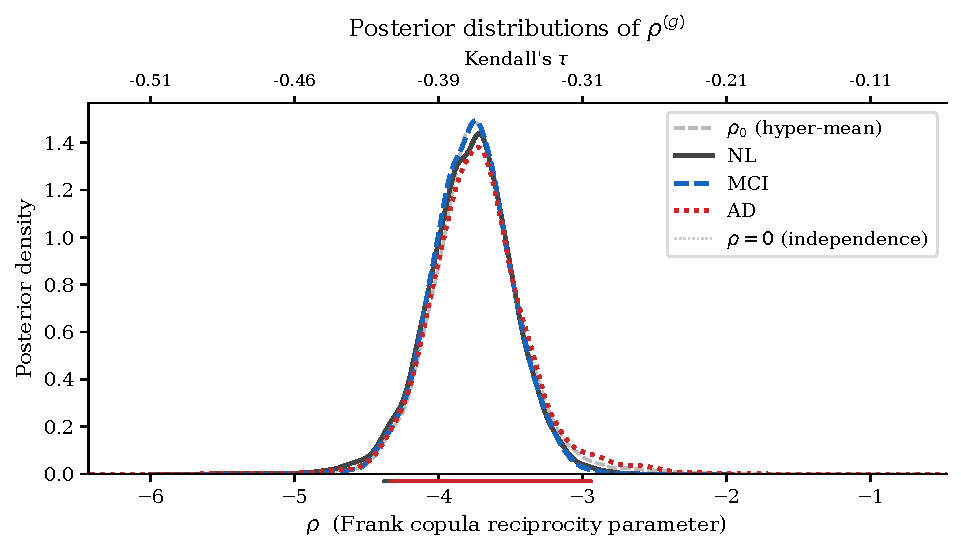
\includegraphics[scale=.65]{Reciprocity.pdf}
\label{fig:reciprocity_cgrg}
%\caption{Reciprocity Parameters for the Three Groups}
\end{center}
\end{figure}



\begin{figure}[htb]
\begin{center}
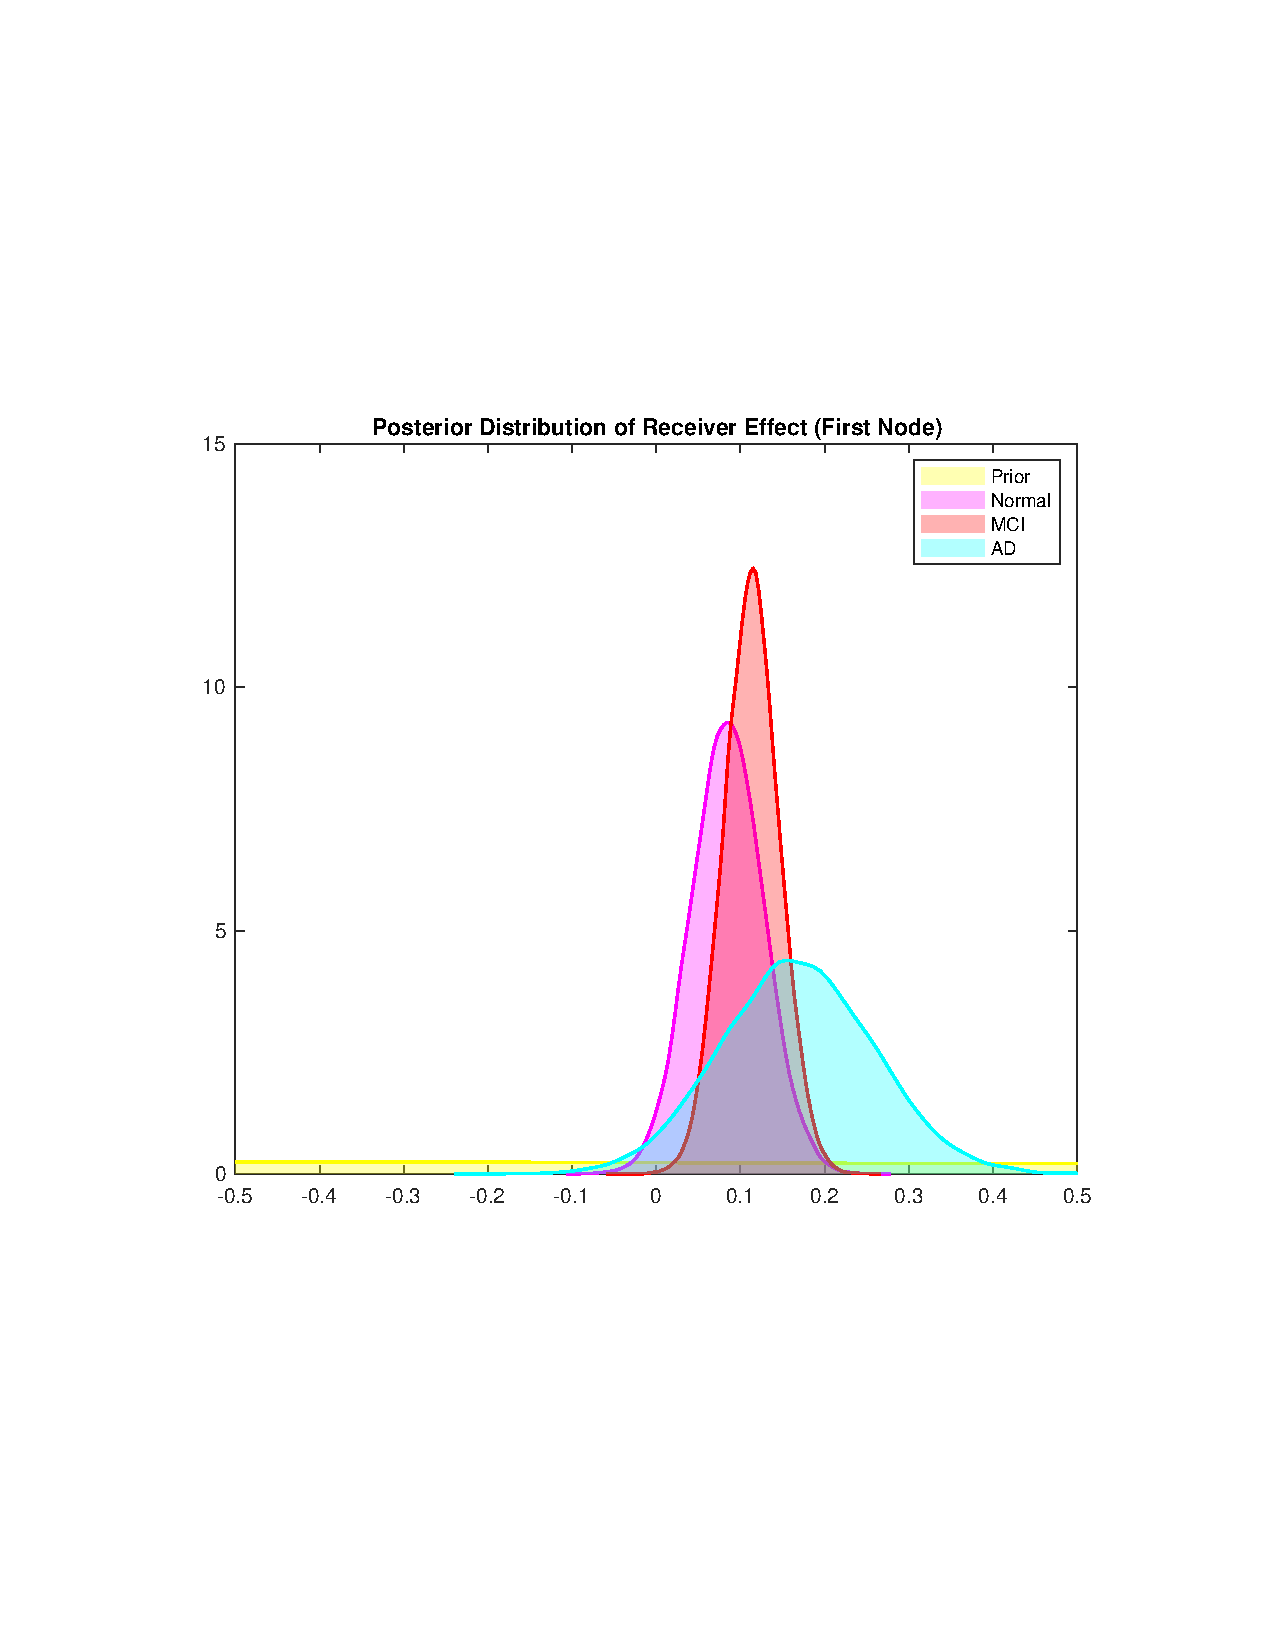
\includegraphics[scale=.65]{receiver_1st.pdf}
\label{fig:receiver_1st_cgrg}
%\caption{Reciprocity Parameters for the Three Groups}
\end{center}
\end{figure}

\begin{figure}[htb]
\begin{center}
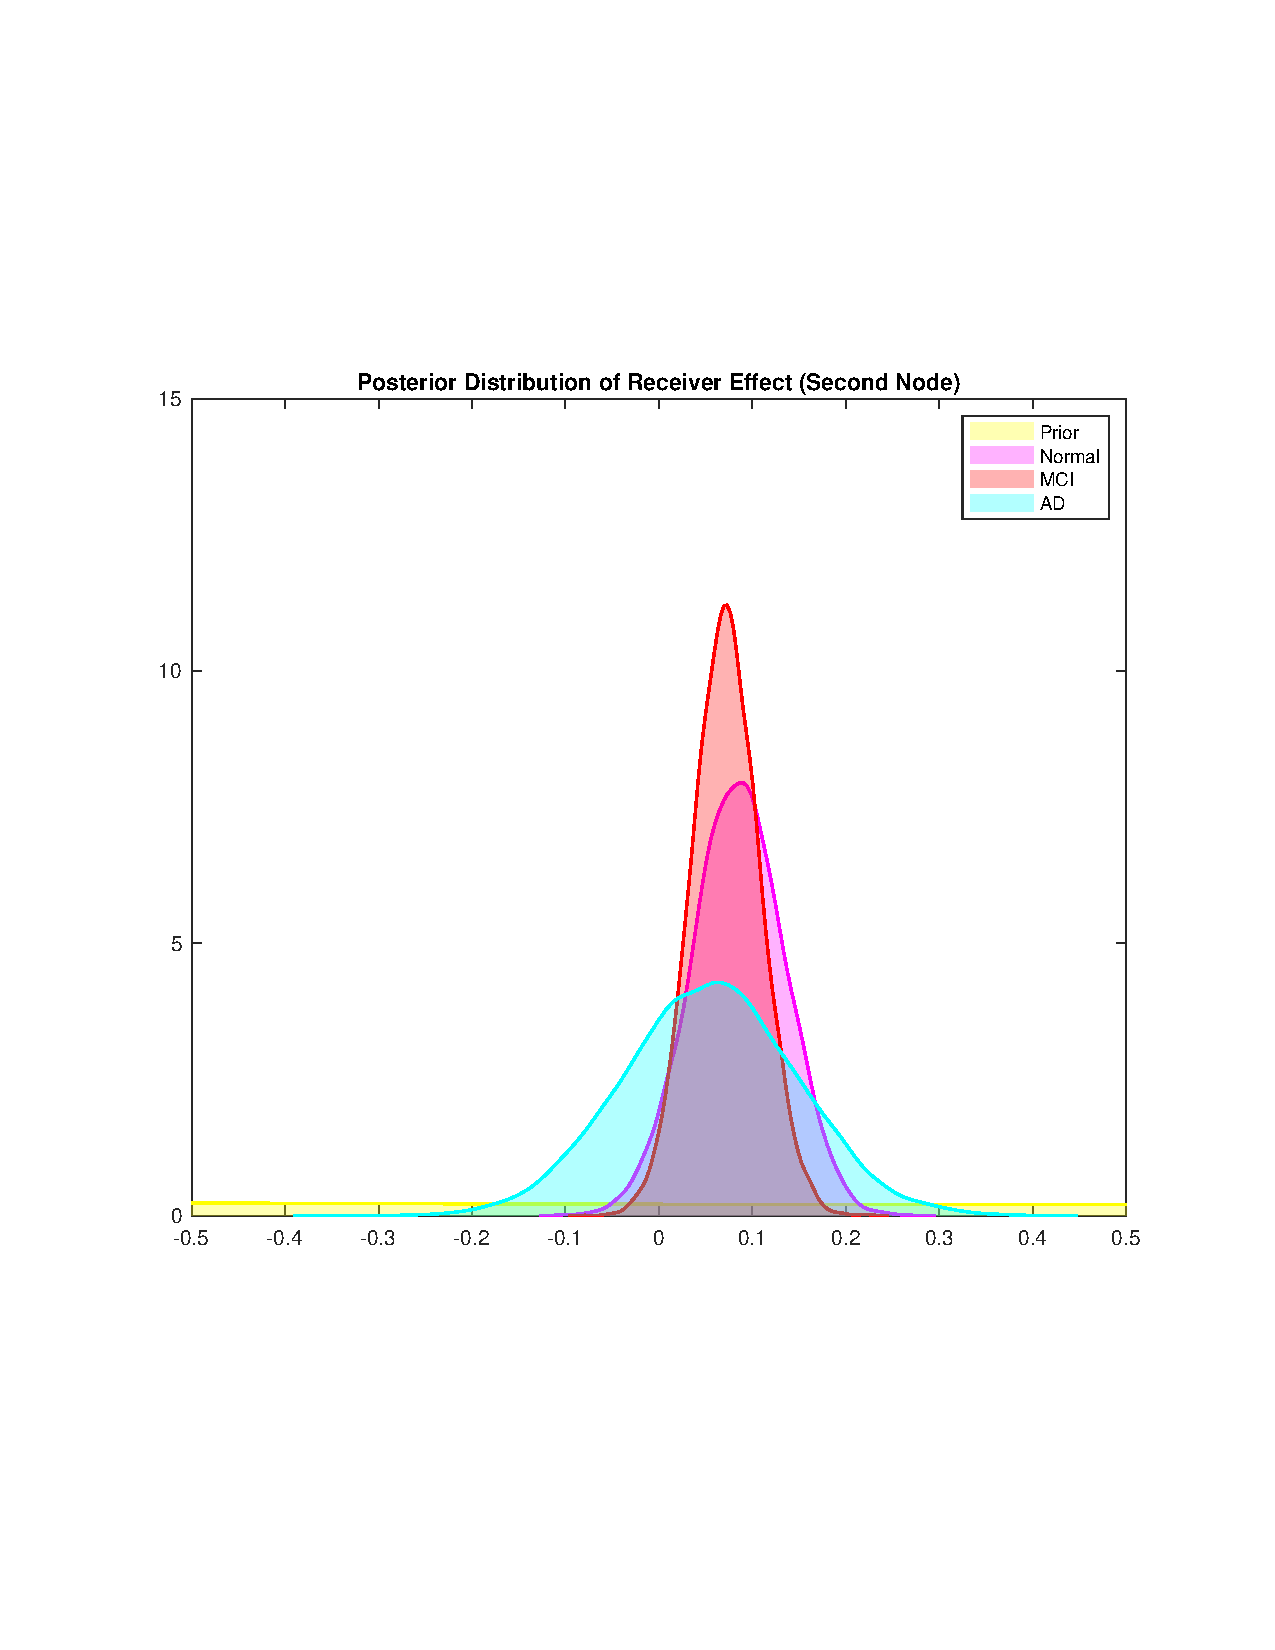
\includegraphics[scale=.65]{receiver_2nd.pdf}
\label{fig:receiver_2nd_cgrg}
%\caption{Reciprocity Parameters for the Three Groups}
\end{center}
\end{figure}

\begin{figure}[htb]
\begin{center}
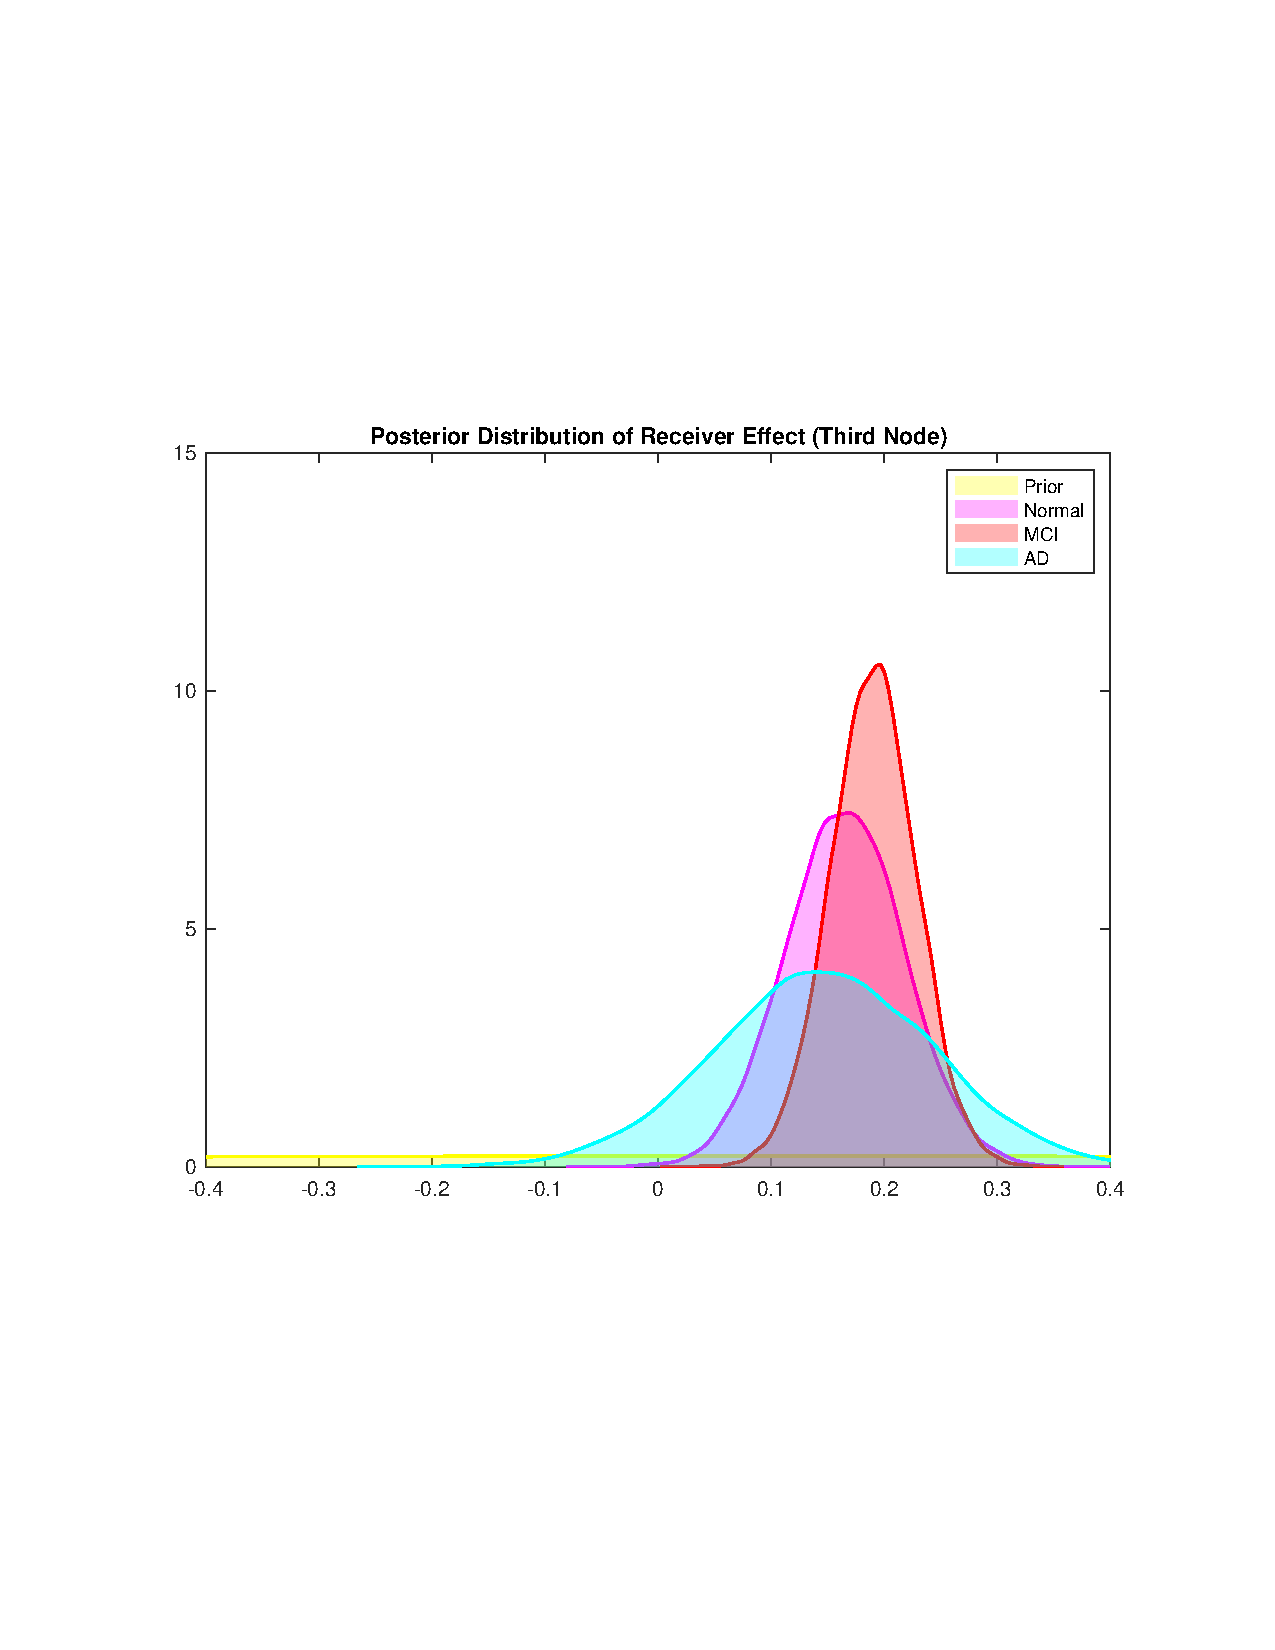
\includegraphics[scale=.65]{receiver_3rd.pdf}
\label{fig:receiver_3rd_cgrg}
%\caption{Reciprocity Parameters for the Three Groups}
\end{center}
\end{figure}

\begin{figure}[htb]
\begin{center}
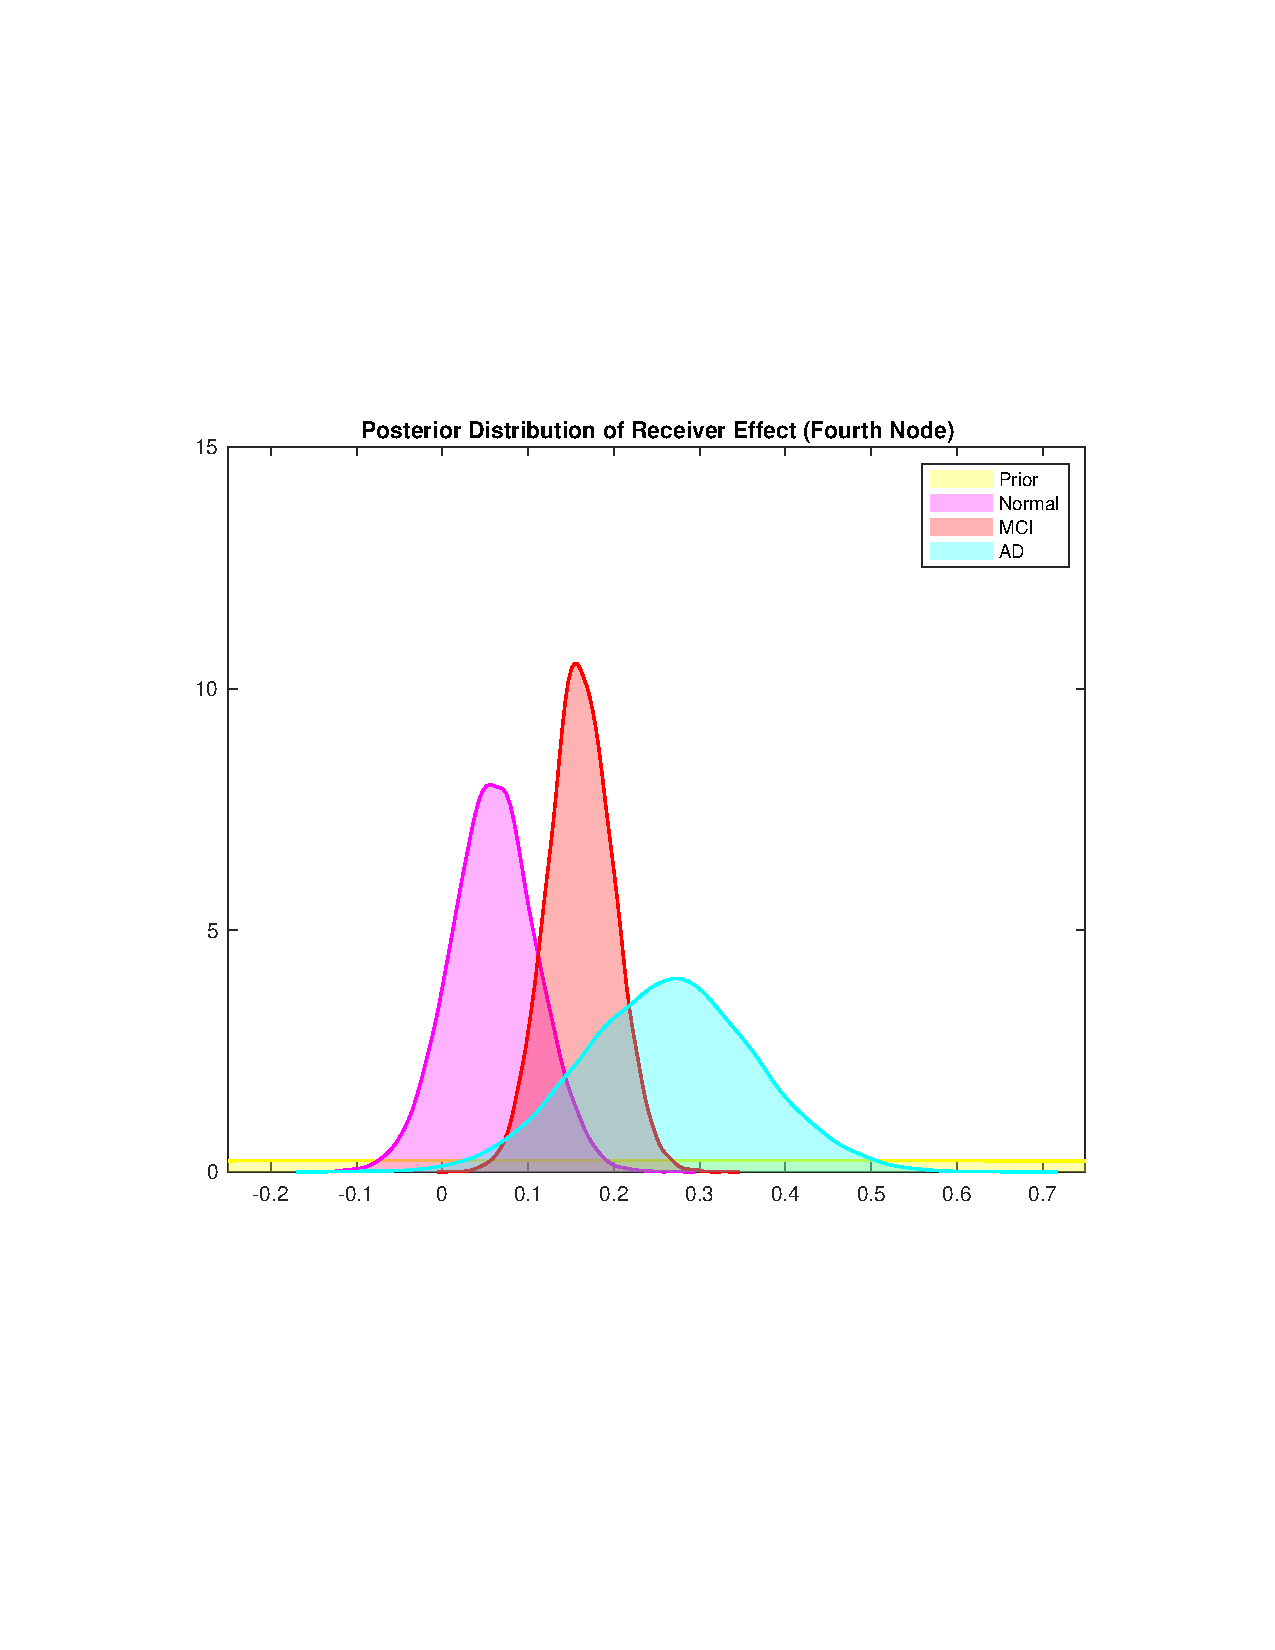
\includegraphics[scale=.65]{receiver_4th.pdf}
\label{fig:receiver_4th_cgrg}
%\caption{Reciprocity Parameters for the Three Groups}
\end{center}
\end{figure}

\begin{figure}[htb]
\begin{center}
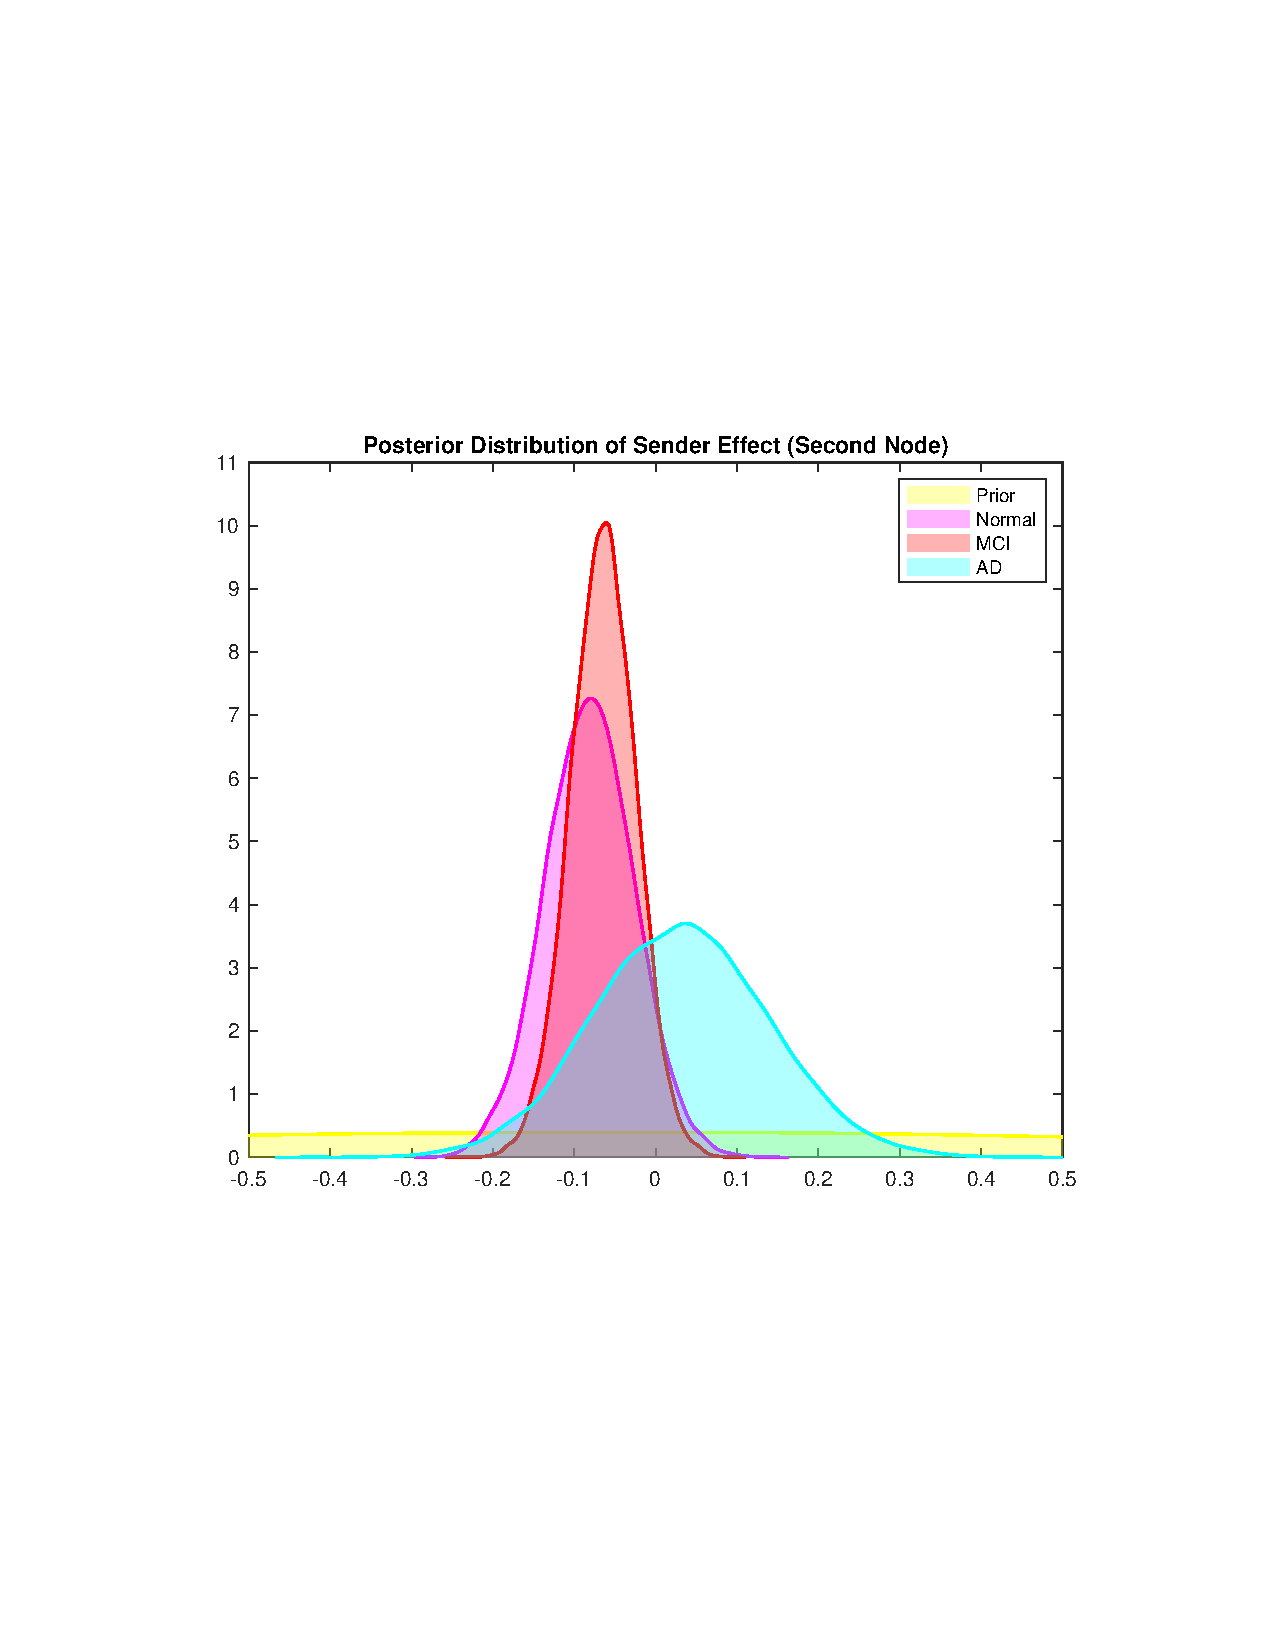
\includegraphics[scale=.65]{sender_2nd.pdf}
\label{fig:sender_2nd_cgrg}
%\caption{Reciprocity Parameters for the Three Groups}
\end{center}
\end{figure}

\begin{figure}[htb]
\begin{center}
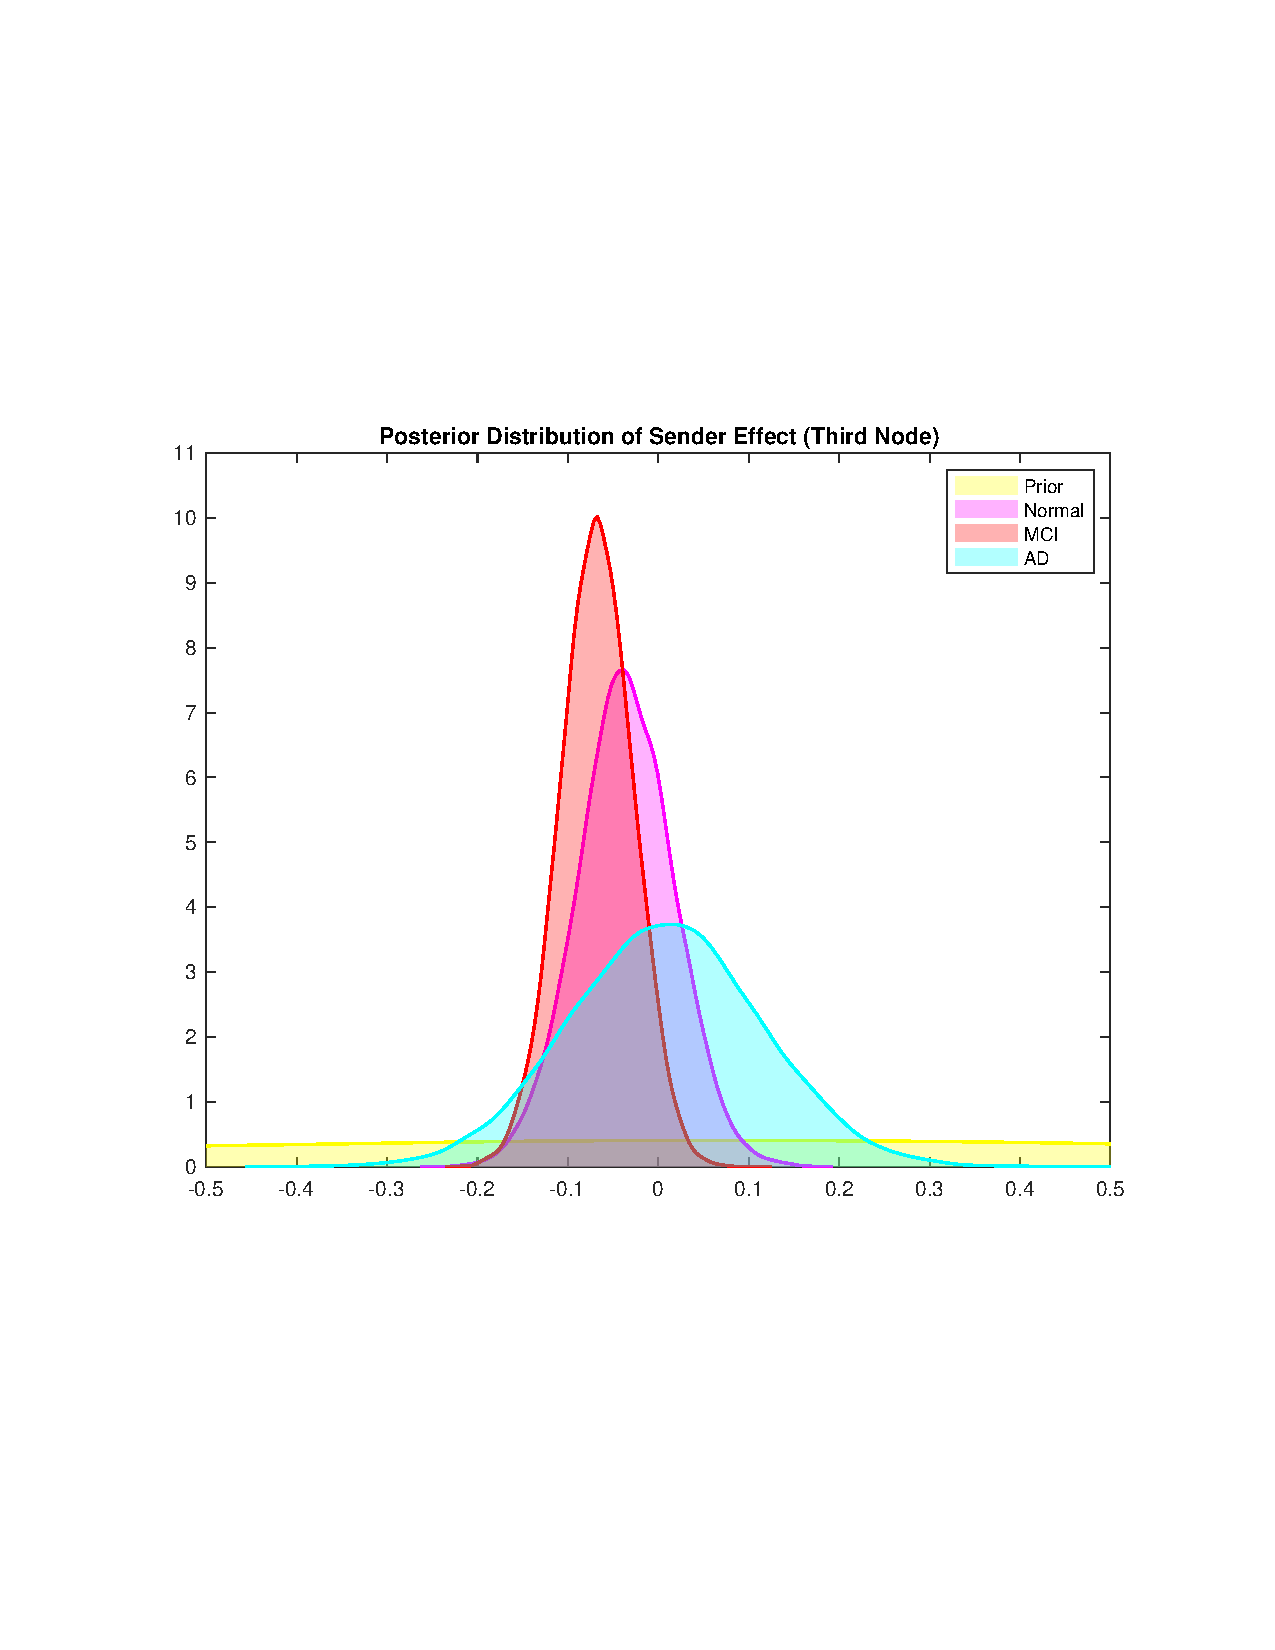
\includegraphics[scale=.65]{sender_3rd.pdf}
\label{fig:sender_3rd_cgrg}
%\caption{Reciprocity Parameters for the Three Groups}
\end{center}
\end{figure}

\begin{figure}[htb]
\begin{center}
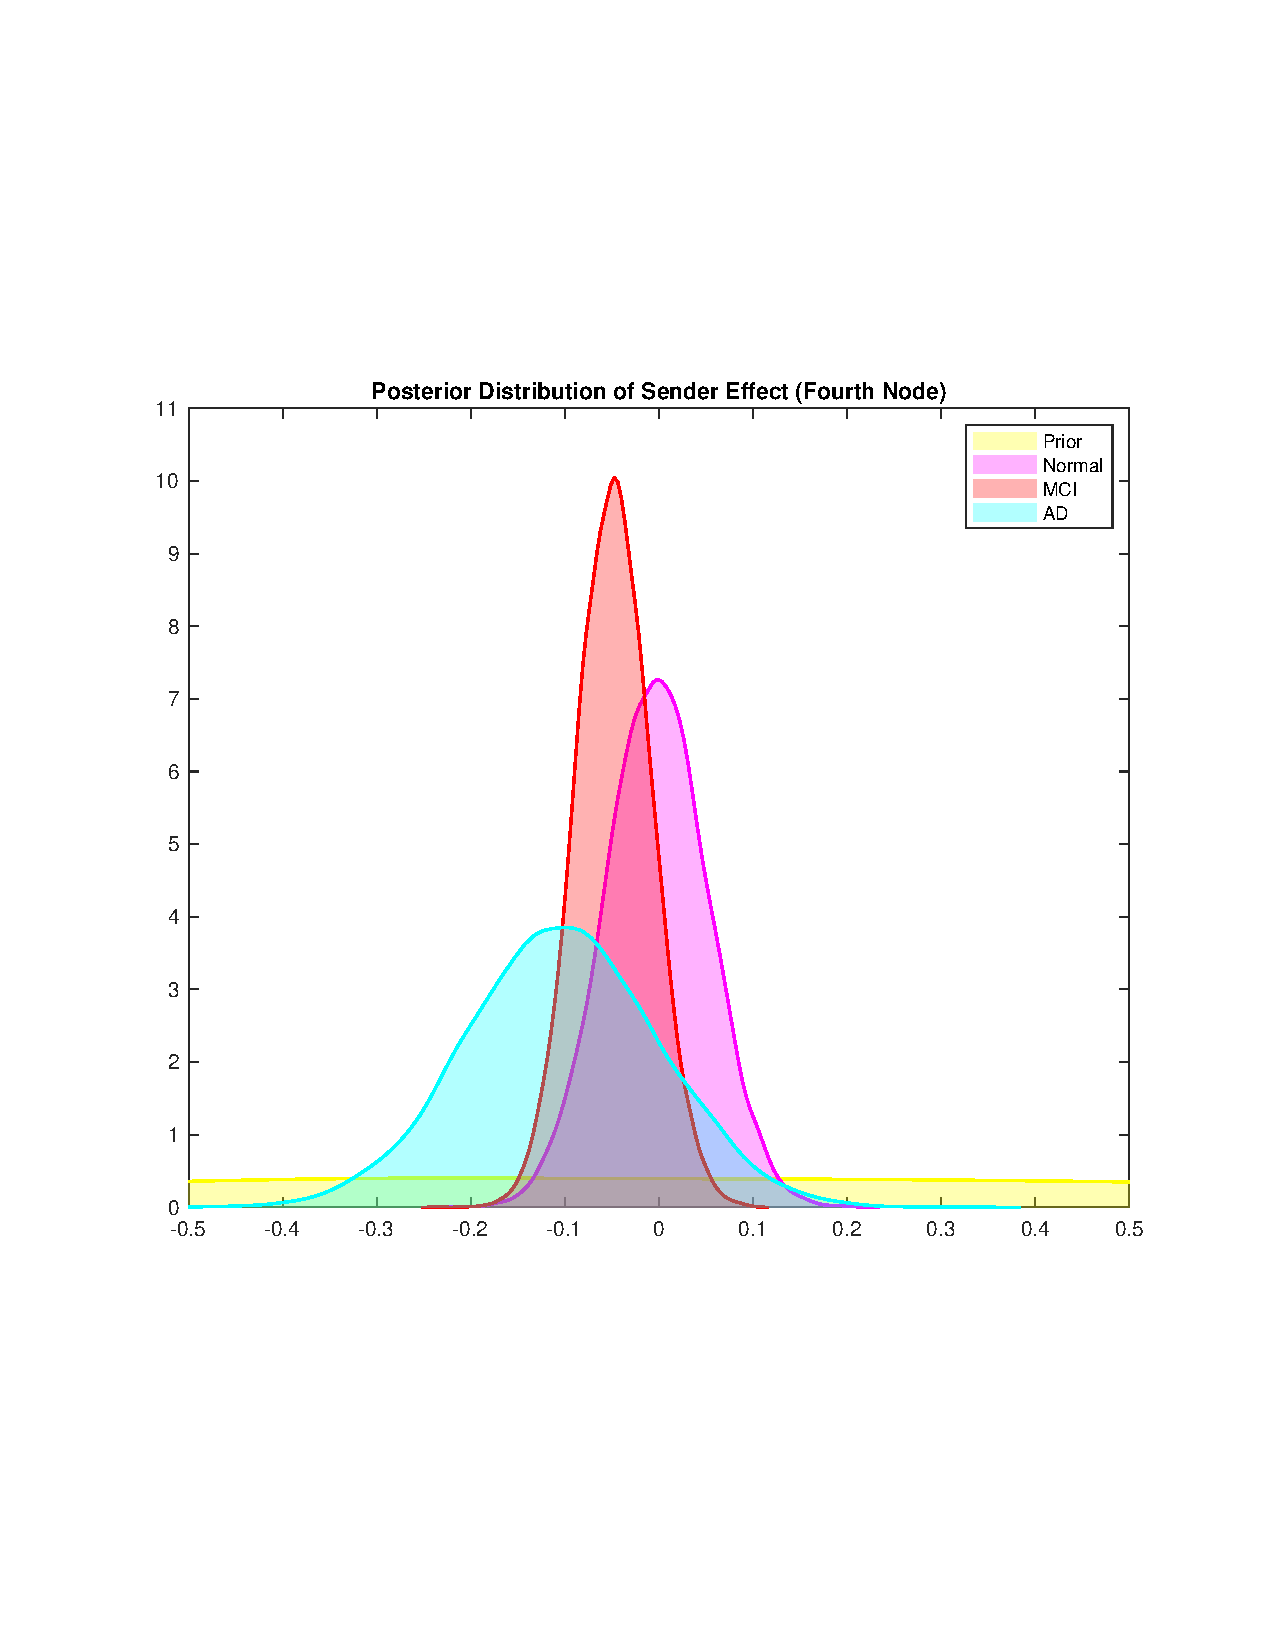
\includegraphics[scale=.65]{sender_4th.pdf}
\label{fig:sender_4th_cgrg}
%\caption{Reciprocity Parameters for the Three Groups}
\end{center}
\end{figure}





%A quick comparison between social networks and brain networks helps determine modeling choices.  In social networks:
%\begin{itemize}
%\item One network is observed for the entire social system.
%\item A single dependence parameter is thought to describe every dyad.
%\end{itemize}
%Whereas, in the present case
%\begin{itemize}
%\item A brain network is observed for each person in the study.
%\item Dependence parameters can be specific to the person or dyad.
%\item This allows for a richer model than the case of a single social network.
%\end{itemize}

%Suppose there are $g=1,\ldots,G$ groups we wish to compare and each group contains $n_g$ subjects.  A hierarchical model specifies
%\begin{align*}
%\rho \sim F(\cdot)
%\end{align*}

\begin{thebibliography}{}
\bibitem{marchini}
Marchini, Jonathan, et al. 
\textit{A new multipoint method for genome-wide association studies by imputation of genotypes.} 
Nature genetics 39.7 (2007): 906.

\bibitem{nie}
Nie, Yunlong, et al. 
\textit{Spectral Dynamic Causal Modelling of Resting-State fMRI: Relating Effective Brain Connectivity in the Default Mode Network to Genetics.} 
arXiv preprint arXiv:1901.09975 (2019).
\end{thebibliography}{}



\end{document}